\documentclass[11pt,letterpaper,english]{article}
\usepackage[T1]{fontenc} % Standard package for selecting font encodings
\usepackage{txfonts} % makes spacing between characters space correctly
\usepackage{xcolor} % Driver-independent color extensions for LaTeX and pdfLaTeX.
\usepackage{hyperref}  %The ability to create hyperlinks within the document
%\usepackage{blindtext} % To create text
%\usepackage{mdwlist} % mdwlist for compact enumeration/list items 
%\usepackage[pagestyles]{titlesec} % related with sections—namely titles, headers and contents
\usepackage{fancyhdr} % header footer placement

\usepackage[top=1in, bottom=1in, left=1in, right=1in] {geometry} % Margins
\usepackage{graphicx}   % Essential for adding images to you document.

\usepackage{sectsty}
\sectionfont{\large}
\subsectionfont{\normalsize}
\subsubsectionfont{\normalsize \it}

\usepackage[font=bf]{caption}% for figure and table captions style
\captionsetup{labelsep=period}

%\setlength{\parskip}{\baselineskip}%
%\setlength{\parindent}{0pt}%


\pagestyle{fancy} % allows you to use the header and footer commands

\raggedright
\begin{document}

\setlength{\parindent}{0in} % Amount of indentation at the first line of a paragraph.

\pagestyle{fancy} \lhead{Revealing the Physics of Galactic Winds with Petascale GPU Simulations} \rhead{Brant Robertson} \renewcommand{%
\headrulewidth}{0.0pt}


\section{PROJECT ACHIEVEMENTS} 

%The project achievements should address the points described below. {\bf This section is typically about 10 pages.} All visual materials, such as charts, graphs, pictures, etc., are included in the page limit; references are {\bf not} included in the page limit. URLs that provide information related to the application should not be included.

Semester 1 of our 2017 INCITE project, "Revealing the Physics of Galactic Winds with Petascale GPU Simulations" resulted in several notable achievements. First and foremost, the project has lead to the single largest hydrodynamic simulation of an isolated galaxy ever performed. With a volume containing over 17 trillion cells, our simulation dwarfs other simulations of this type by over an order of magnitude. In order to perform this simulation, our project utilized 8096 GPUs on \textit{Titan} for a total of $\sim$8 million core-hours. The simulation was the culmination of our work in Semester 1 which included generating specialized initial conditions for a stable galaxy model, implementing a supernova feedback scheme to drive a wind from the galaxy, and improving the hydrodynamics algorithms and other physics available in our GPU-based code \textit{Cholla}. Each of these accomplishments is described in further detail in the sections below.

\subsection{Significance of Accomplishments to Date} 

%Explain what advances you accomplished through the INCITE award (impact on community paradigms, valuable insights into or solving a long-standing challenge, etc.). Place the proposed research in the context of competing work in your discipline or business. Reiterate the milestones of your proposal and discuss the accomplishments (planned or unplanned) achieved this year relative to those milestones and allocation use (Section 1aii). Summarize the impact of the results achieved: What conclusions can be drawn, and what is solved because of these results? What new and follow-on investigations have these results motivated?

Our 2016 INCITE proposal focused on the role that radiatively-cooling galactic winds may play in galaxy evolution. While observations routinely show fast ($v > 1000$ km/s), cool ($T\sim10^4$ K) winds being driven out of galaxies with high rates of star formation, numerical simulations of galaxies have thus far failed to reproduce them. Cosmological simulations lack the resolution required to generate the winds, and high-resolution simulations lack the volume to track gas once it has been driven out of the galaxy. Our project aims to bridge this gap by producing high resolution simulations of disk galaxies that span a sufficient distance from the wind-generation region within galaxies to demonstrate whether starburst-driven winds can cool in the manner suggested by recent theoretical work.

In order to carry out the simulations described in our proposal, a number of preparatory efforts were completed in the first semester. In Tables 1 and 2, we reproduce the research objectives and milestones from our 2016 proposal. We expand on the current status of each objective and related achievements in the following subsections.

\begin{table}[h]
%\centering
\vspace{-.12in}
\begin{tabular}{|l|l|} 
\multicolumn{2}{l}{\bf{Table 1: Research Objectives}}\\
\hline
\textbf{RO.A} & Simulate galactic outflows with numerical models that allow for supersonic
wind velocities. \\ \hline
\textbf{RO.B} & Quantify the importance of radiative cooling 
for the multiphase structure of observed galactic outflows.\\ \hline
\textbf{RO.C} & Determine the mass and energy coupling of ISM gas to supernova-driven outflows.\\
\hline
\end{tabular}
\end{table}


\begin{table}[h]
%\centering
\vspace{-.12in}
\begin{tabular}{|l|p{4.6in}|l|} 
\multicolumn{3}{l}{\bf{Table 2: Research Milestones}}\\
\hline
\multicolumn{2}{|l|}{\bf Milestone} & {\bf Objective} \\ \hline
\multicolumn{3}{|c|}{\it Semester 1} \\ \hline
\textbf{RM.A} & Create and test initial conditions for galactic disk simulations. & RO.A \\ \hline
\textbf{RM.B} & Implement and calibrate feedback model for driving galactic outflows. & RO.A\\ \hline
\multicolumn{3}{|c|}{\it Semester 2} \\ \hline
\textbf{RM.C} & Model the multiphase structure and radiative cooling of galactic
outflows on $\sim10$kpc scales. & RO.A, RO.B \\ \hline
\multicolumn{3}{|c|}{\it Semester 3} \\ \hline
\textbf{RM.D} & Determine the role of full three-dimensionality on the velocity and density
structure of galactic outflows. & RO.A, RO.B\\ \hline
\multicolumn{3}{|c|}{\it Semester 4} \\ \hline
\textbf{RM.E} & Simulate galactic outflows at large dynamic range to generate {\it ab initio} $\sim10$kpc-scale winds from $\sim$pc-scale supernovae bubbles. & RO.A, RO.B, RO.C\\ 
\hline
\end{tabular}
\end{table}

\subsubsection{Research Milestone A: Create and test initial conditions for galactic disk simulations}

The first major accomplishment of our project is the successful creation of an initial conditions generator for our global galactic disk simulations. Implemented as a module in our code, \textit{Cholla}, the initial conditions for these simulations consist of a $10^4$ K isothermal gas disk that is placed in vertical hydrostatic equilibrium with a background potential. The background potential consists of a Miyamoto-Nagai disk that represents the gaseous and stellar components of the galaxy, plus a Navarro-Frenk-White halo profile that accounts for the dark matter contribution to the potential. The disk is initially set to be differentially rotating, with the velocity gradient balancing the radial pressure profile. In addition to a disk, our initial conditions also contain a gaseous halo. The halo is set to be in adiabatic hydrostatic equilibrium with the background potential, which prevents it from collapsing onto the disk.

\begin{figure}[h]
\centering
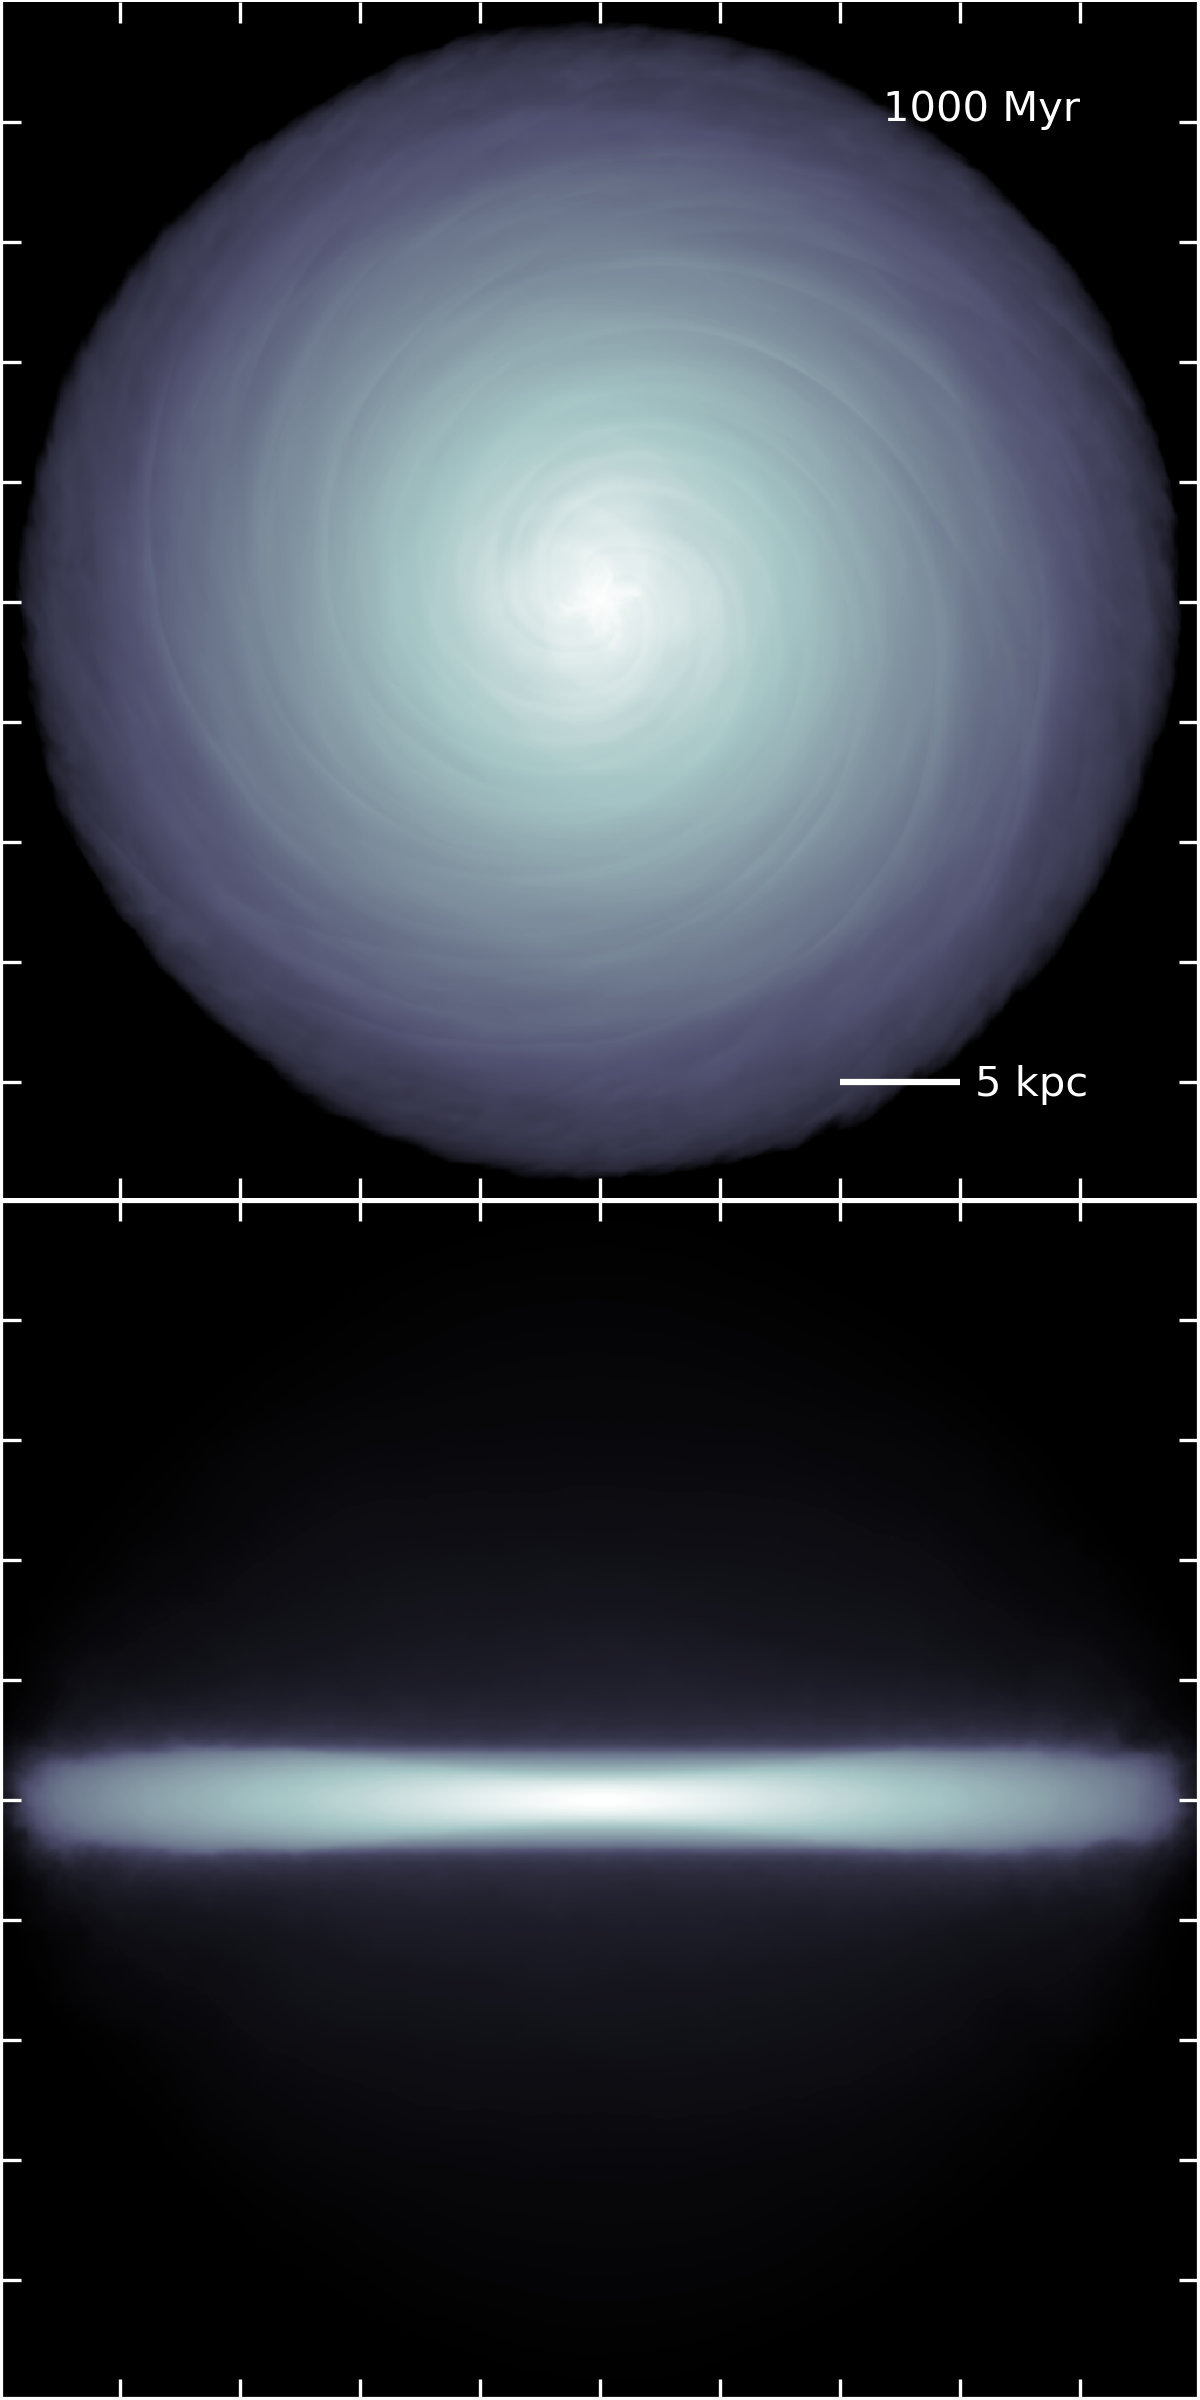
\includegraphics[width=0.35\linewidth]{MW_d.png}
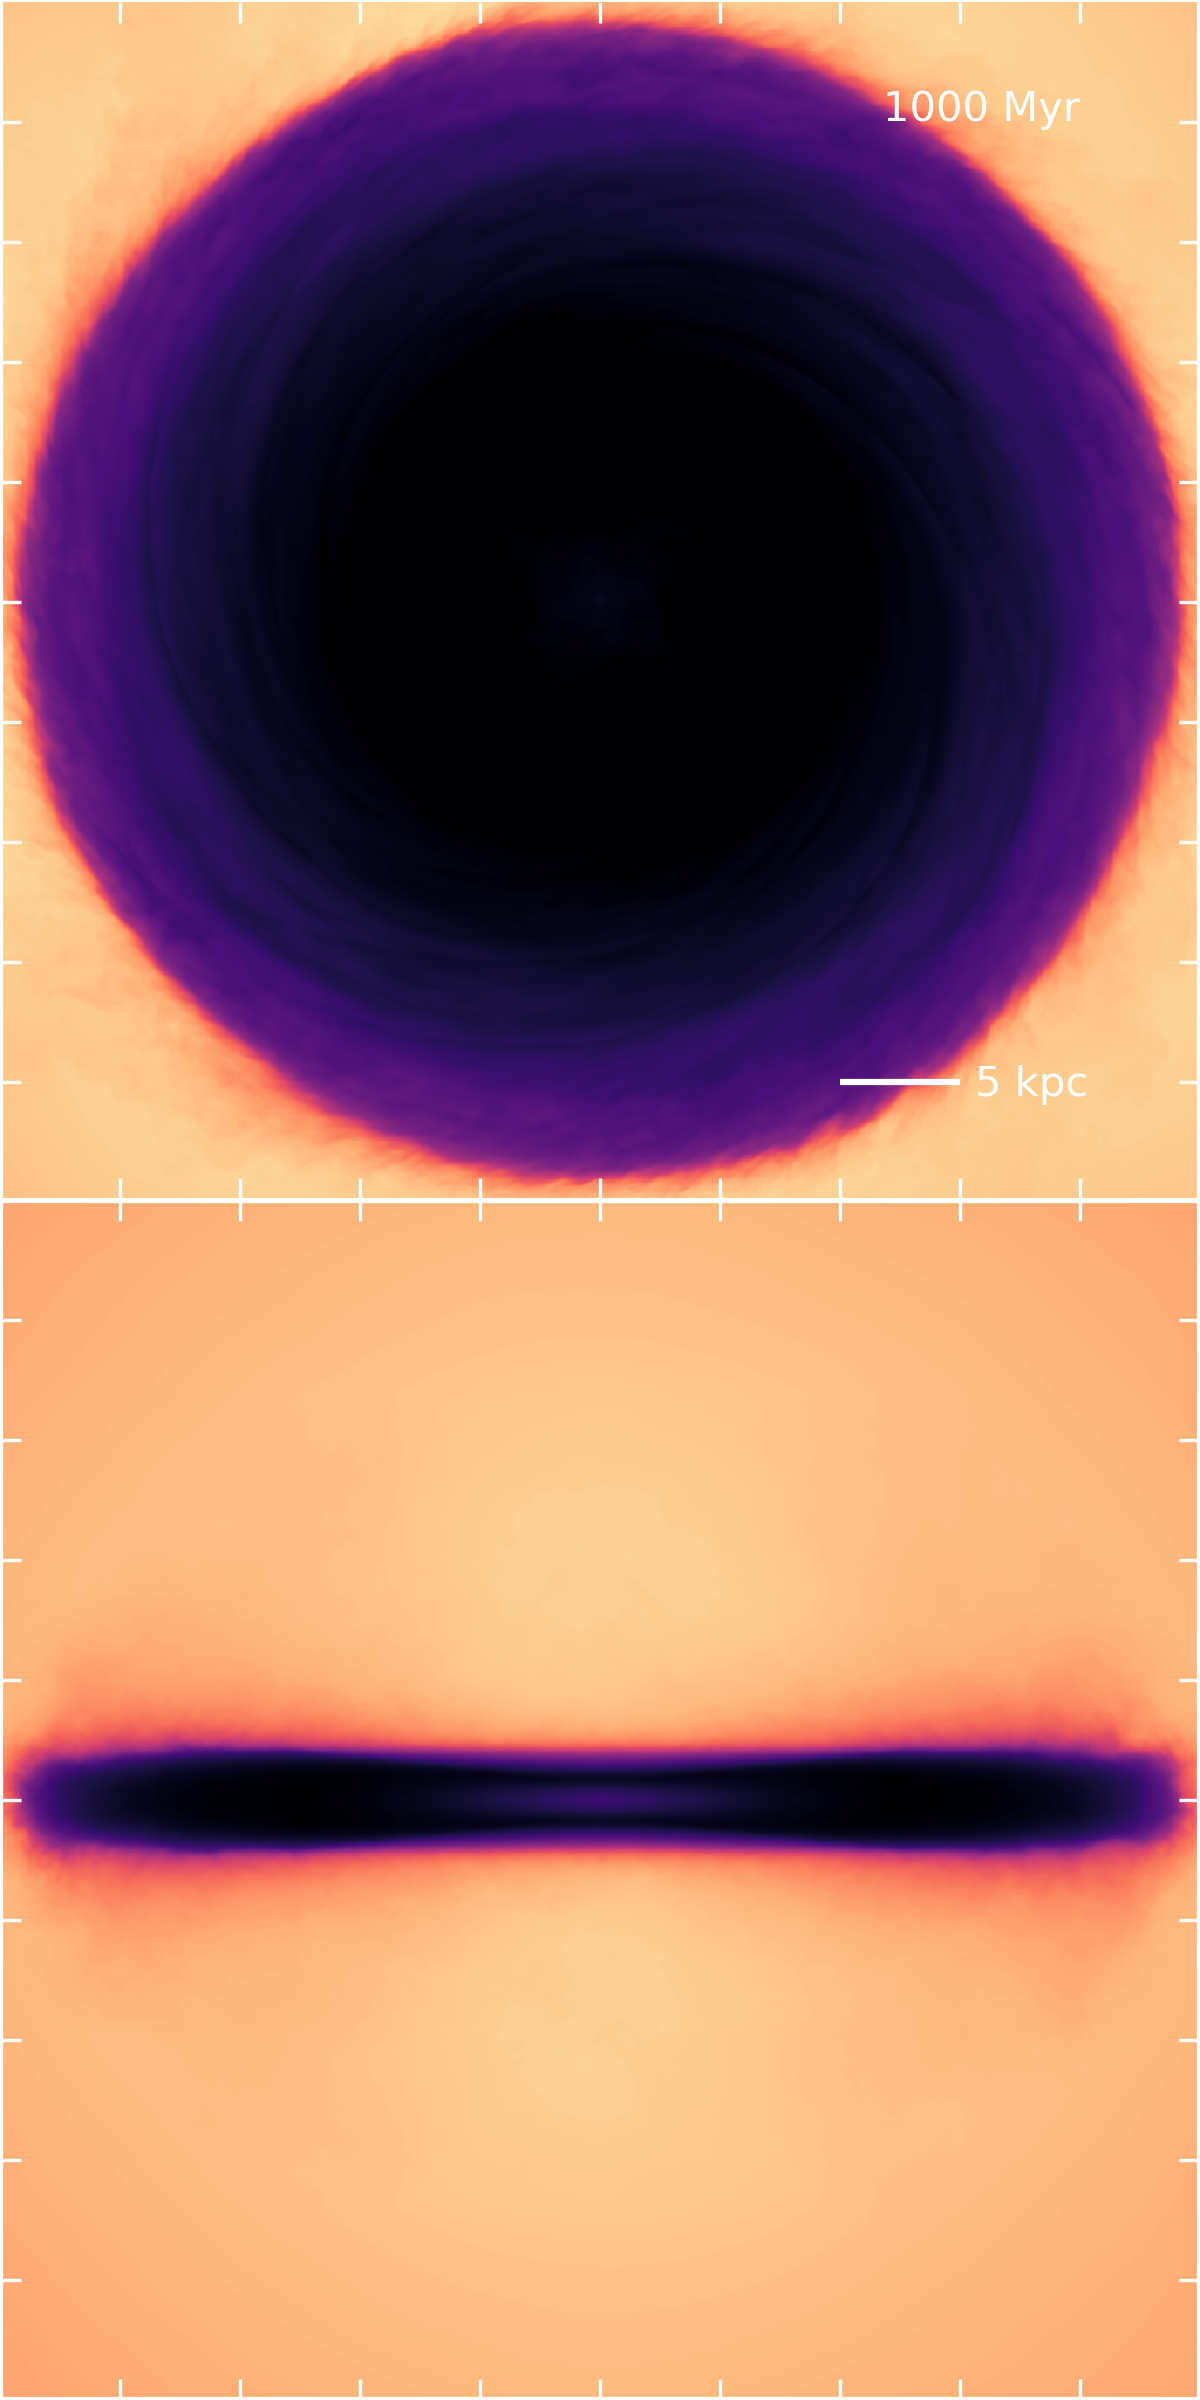
\includegraphics[width=0.35\linewidth]{MW_T.png}
\caption{Figure caption.}
\label{fig:MW_ICs}
\end{figure}

We have created two versions of these initial conditions, one with parameters representative of a Milky-Way-like galaxy, and one with parameters that mimic those of the nearby starburst galaxy M82. An example of the Milky Way galaxy after 1 Gyr of evolution is shown in Figure \ref{fig:MW_ICs}. The left panels show projected gas density in the x-y and x-z planes, while the right panels show projected gas temperature. After many millions of years of evolution, the differential rotation of the gas in the disk leads to the spiral features that can be seen in the x-y density projection. A small amount of turbulence is generated on the surface of the disk due to the shear between disk and halo gas (only the disk gas is given an initial rotation). Otherwise, the disk and halo look almost identical to their initial setup.
Adiabatic simulations using both versions of the initial conditions have demonstrated that they are stable for at least a gigayear, far longer than our wind simulations will be run. Compared to similar projects in the literature, our initial conditions are highly specialized (see e.g. Cooper et al. 2008, Fielding et al. 2017). Most models simply use an isothermal disk with no halo, or an isothermal halo. When experimenting with our initial conditions, we found that isothermal halo models were not stable over the long term. In addition, our simulations require the presence of an initial halo to determine the effect that swept-up hot halo gas may have on the evolution of galactic winds. Thus, our highly specialized initial conditions represent a necessary advancement of the field.

\subsubsection{Research Milestone B: Implement and calibrate feedback model for driving galactic outflows}

The second major accomplishment of our program is a unique implementation of a supernova feedback model that will allow us to test the premise that supernova-driven winds can cool radiatively at large radii. The theoretical studies that our project aims to test are extensions to the 1985 supernova-driven wind model of Chevalier \& Clegg. This model, hereafter referred to as CC85, posits that a constant deposition of mass and energy within a spherical region in the center of a galaxy should result in a spherically-expanding flow of gas outward. Exact solutions for the density, velocity, and pressure of the wind can be calculated as a function of radius. Neither radiative cooling of the wind nor the effect of a gravitational potential are considered in the CC85 model. Despite this, X-ray observations indicate that the CC85 model is a good fit for the central region of the superwind in M82 (Strickland \& Heckman, 2009).

More recent models have extended the CC85 model to include the effects of both gravity (Wang 1995) and radiative cooling (Wang 2005, Thompson 2016). These models suggest that given sufficient mass-loading of the hot wind, dramatic cooling can take place at radii 1 - 10 kpc from the wind-generation radius, which could account for the fast-moving, cool gas observed around starburst galaxies. In order to efficiently test this cooling model, we have created a supernova feedback model that matches the CC85 model as closely as possible. In Year 2, we will extend this model to incorporate more realistic versions of supernova feedback.

Our current feedback model assumes a constant rate of mass and energy injection within the starburst radius, with the mass and energy injection set by three parameters: the star formation rate, the mass-loading factor, and the supernova thermalization efficiency. Our initial models use reasonable parameters for the past star formation rate, mass-loading, and supernova thermalization efficiency as calculated from observations of M82. The resulting wind can then be compared against the theoretically-calculated model, as shown in \ref{fig:CC85}.

\begin{figure}[h]
\centering
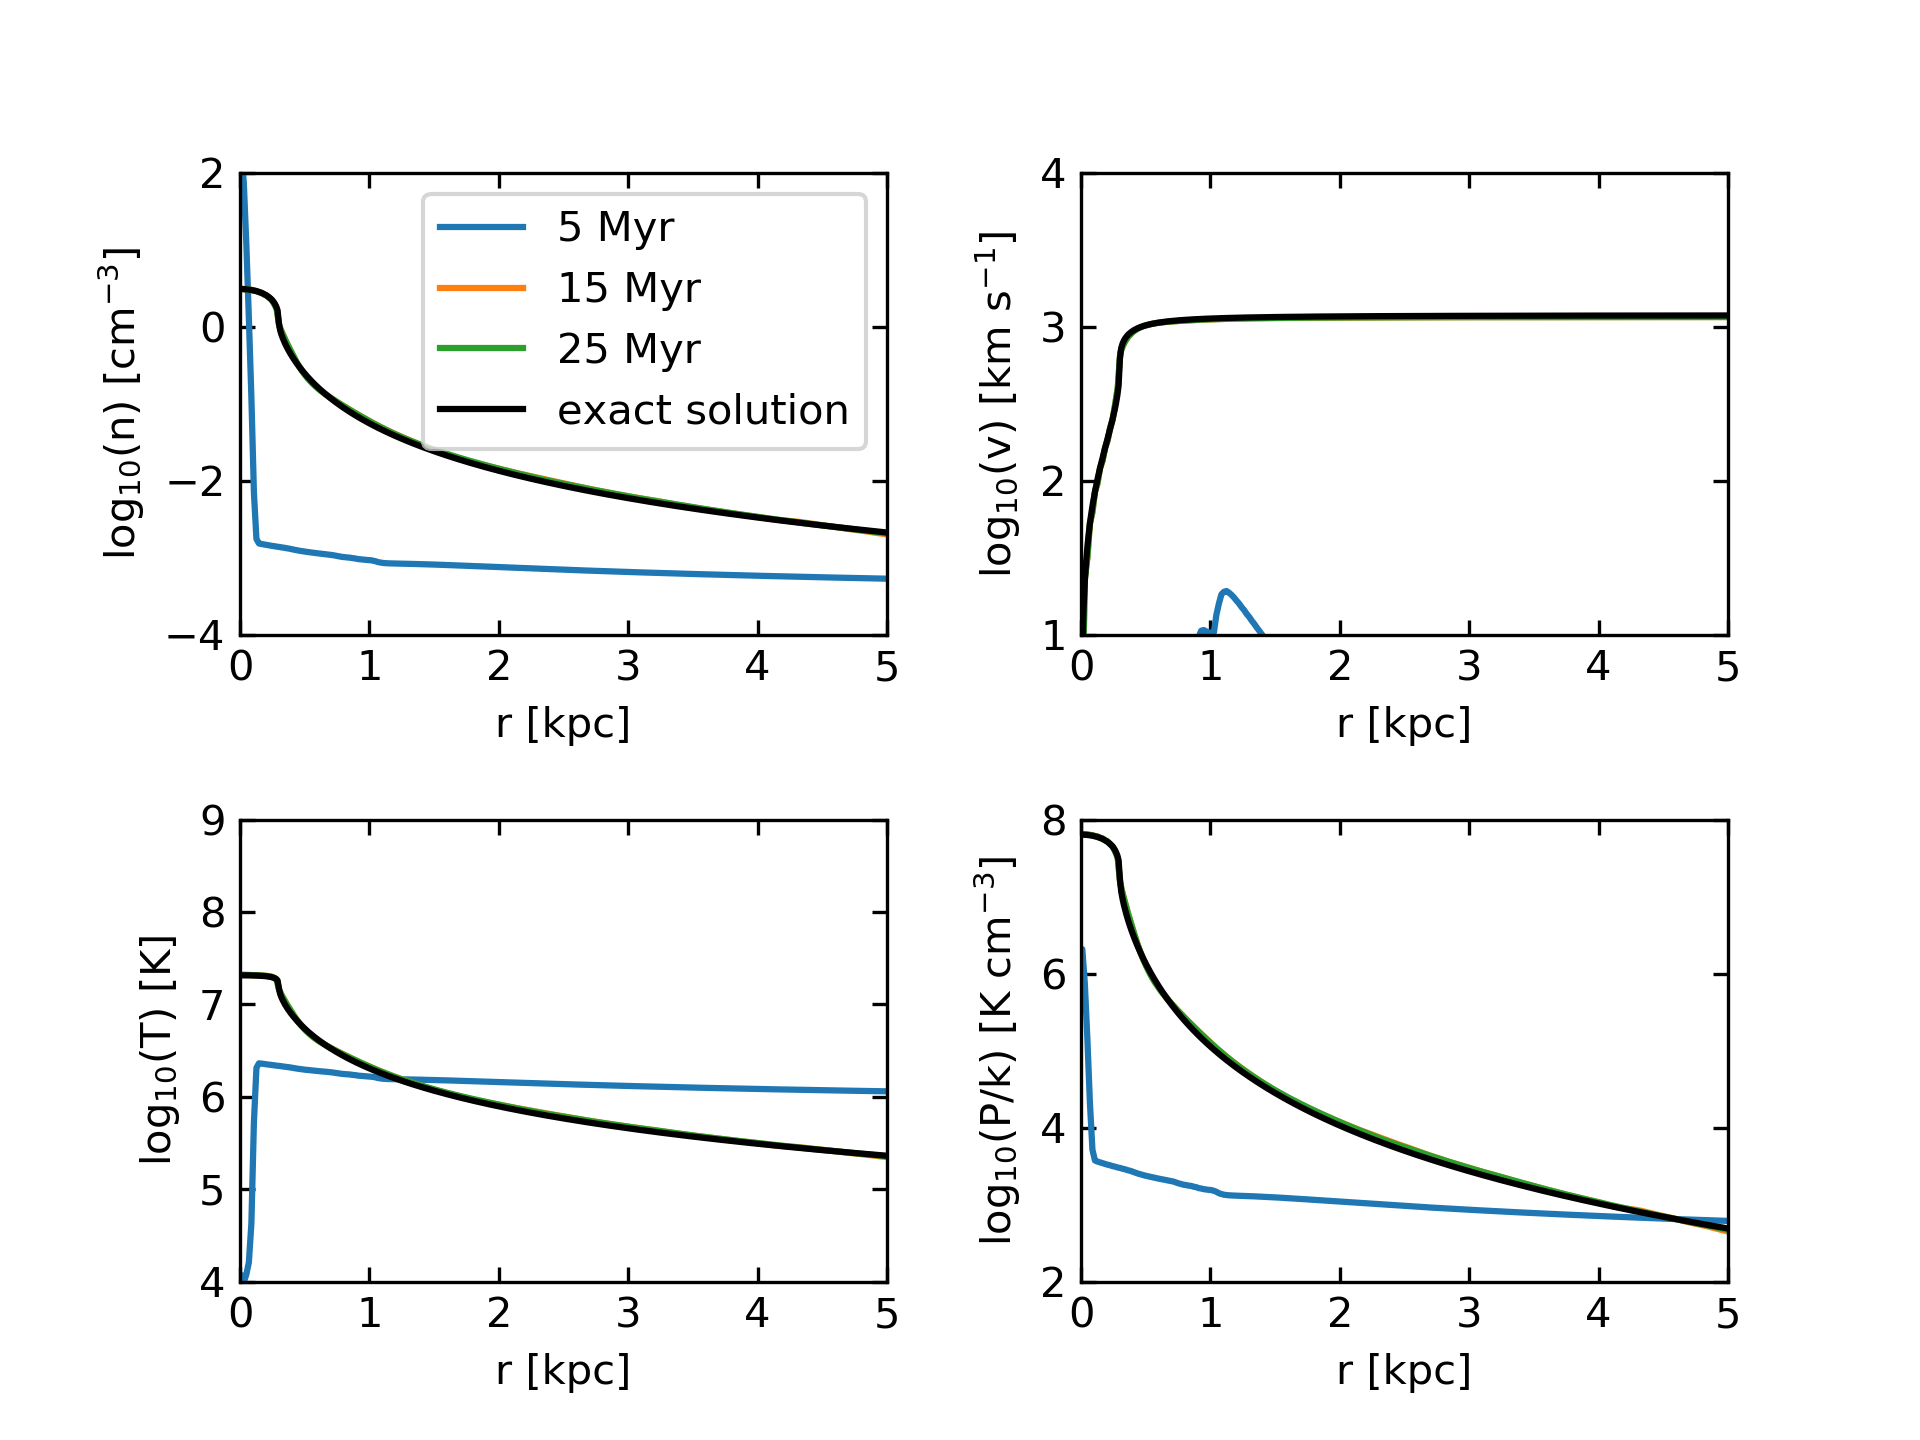
\includegraphics[width=0.8\linewidth]{CC85.png}
\caption{Figure caption.}
\label{fig:CC85}
\end{figure}

Our fiducial model uses a star formation rate of 20 $M_\odot$/yr, a mass-loading factor of $\beta = 1.4$, and a supernova thermalization efficiency of $\alpha = 0.9$. \ref{fig:CC85} displays the density, velocity, temperature, and pressure of the resulting wind as a function of radius. Plotted in this figure are both the exact solution (black line), as well as the values along the $z$-axis of one of our calibration simulations at 5, 15, and 25 Myr. We start the supernova feedback after 5 Myr, so the blue line is representative of the values of our initial conditions. The orange and green lines are difficult to detect, because they lie \textit{directly} underneath the exact solution, demonstrating that within 10 million years, this feedback model has set up a stable wind with outflow parameters that match those expected. (Note that this is a simulation \textit{without} radiative cooling. This figure represents an achievement both for the CC85 analytic model, as well as for our code \textit{Cholla}.

As a control for our radatively-cooling wind simulations, we have run a production-scale adiabatic simulation with these fiducial parameters. Our production simulation are run on grids with $2048\times2048\times2048$ cells, in a domain with dimensions 5 kpc $\times$ 5 kpc $\times$ 10 kpc, giving a resolution of 4.9 pc at all locations in the simulation volume. Density and temperature projections for this adiabatic control simulation after 30 million years of evolution are shown in Figure \ref{fig:adiabatic_2048}. The biconical outflow driven by the central energy and mass input is clearly visible in the temperature projection, as is the fall-off in temperature with radius due to the expansion of the flow. The energy injection has resulted in the blow-out of all of the gas from the central region of the disk. This simulation represents by far the largest hydrodynamic simulation of an isolated galaxy ever performed, and its hydrodynamic resolution tops that of even the current largest cosmological simulations (e.g. the IllustrisTNG simualtion, which has $\sim$15 million hydrodynamic particles, vs. our $\sim$17 million cells). Thus, despite the fact that this is merely our control simulation, it represents a major achievement and technological milestone for our program.

\begin{figure}[h]
\centering
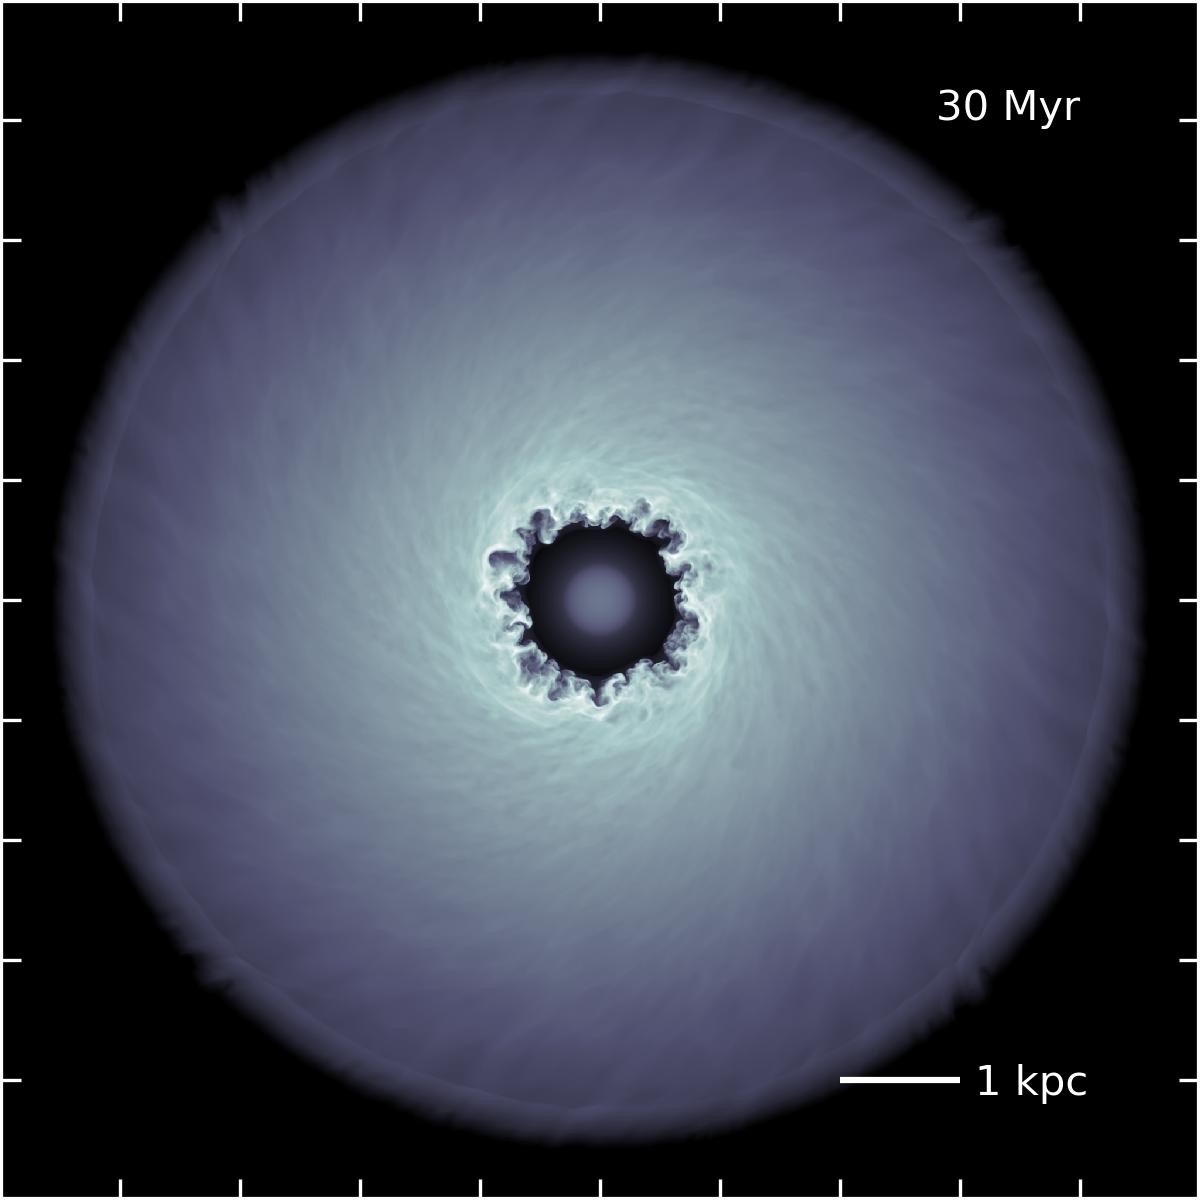
\includegraphics[width=0.35\linewidth]{M82_dxy.png}
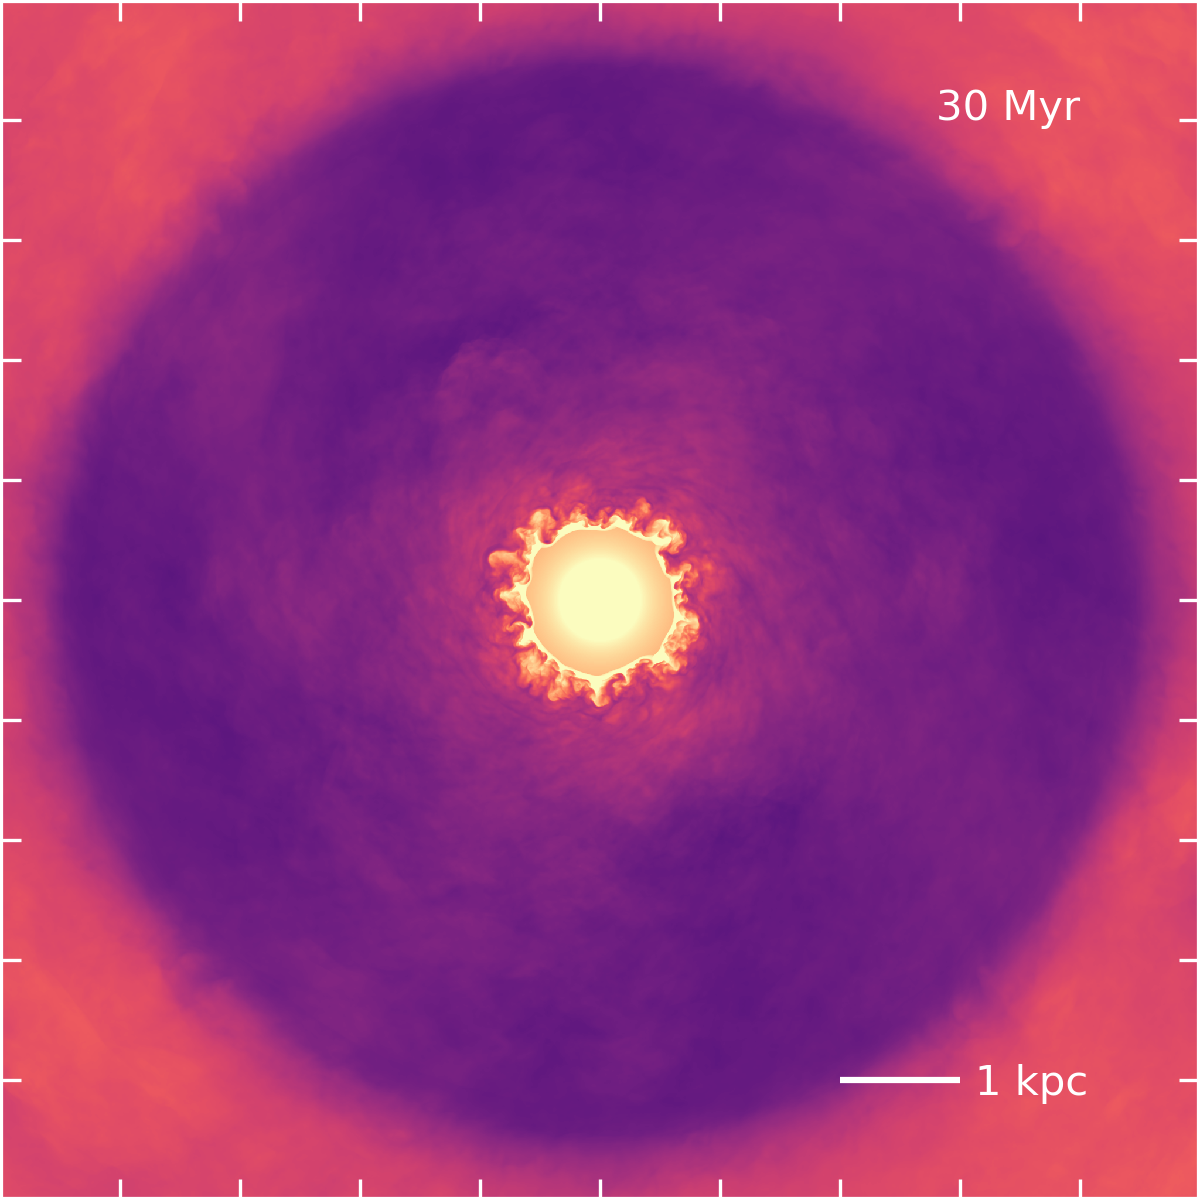
\includegraphics[width=0.35\linewidth]{M82_Txy.png}
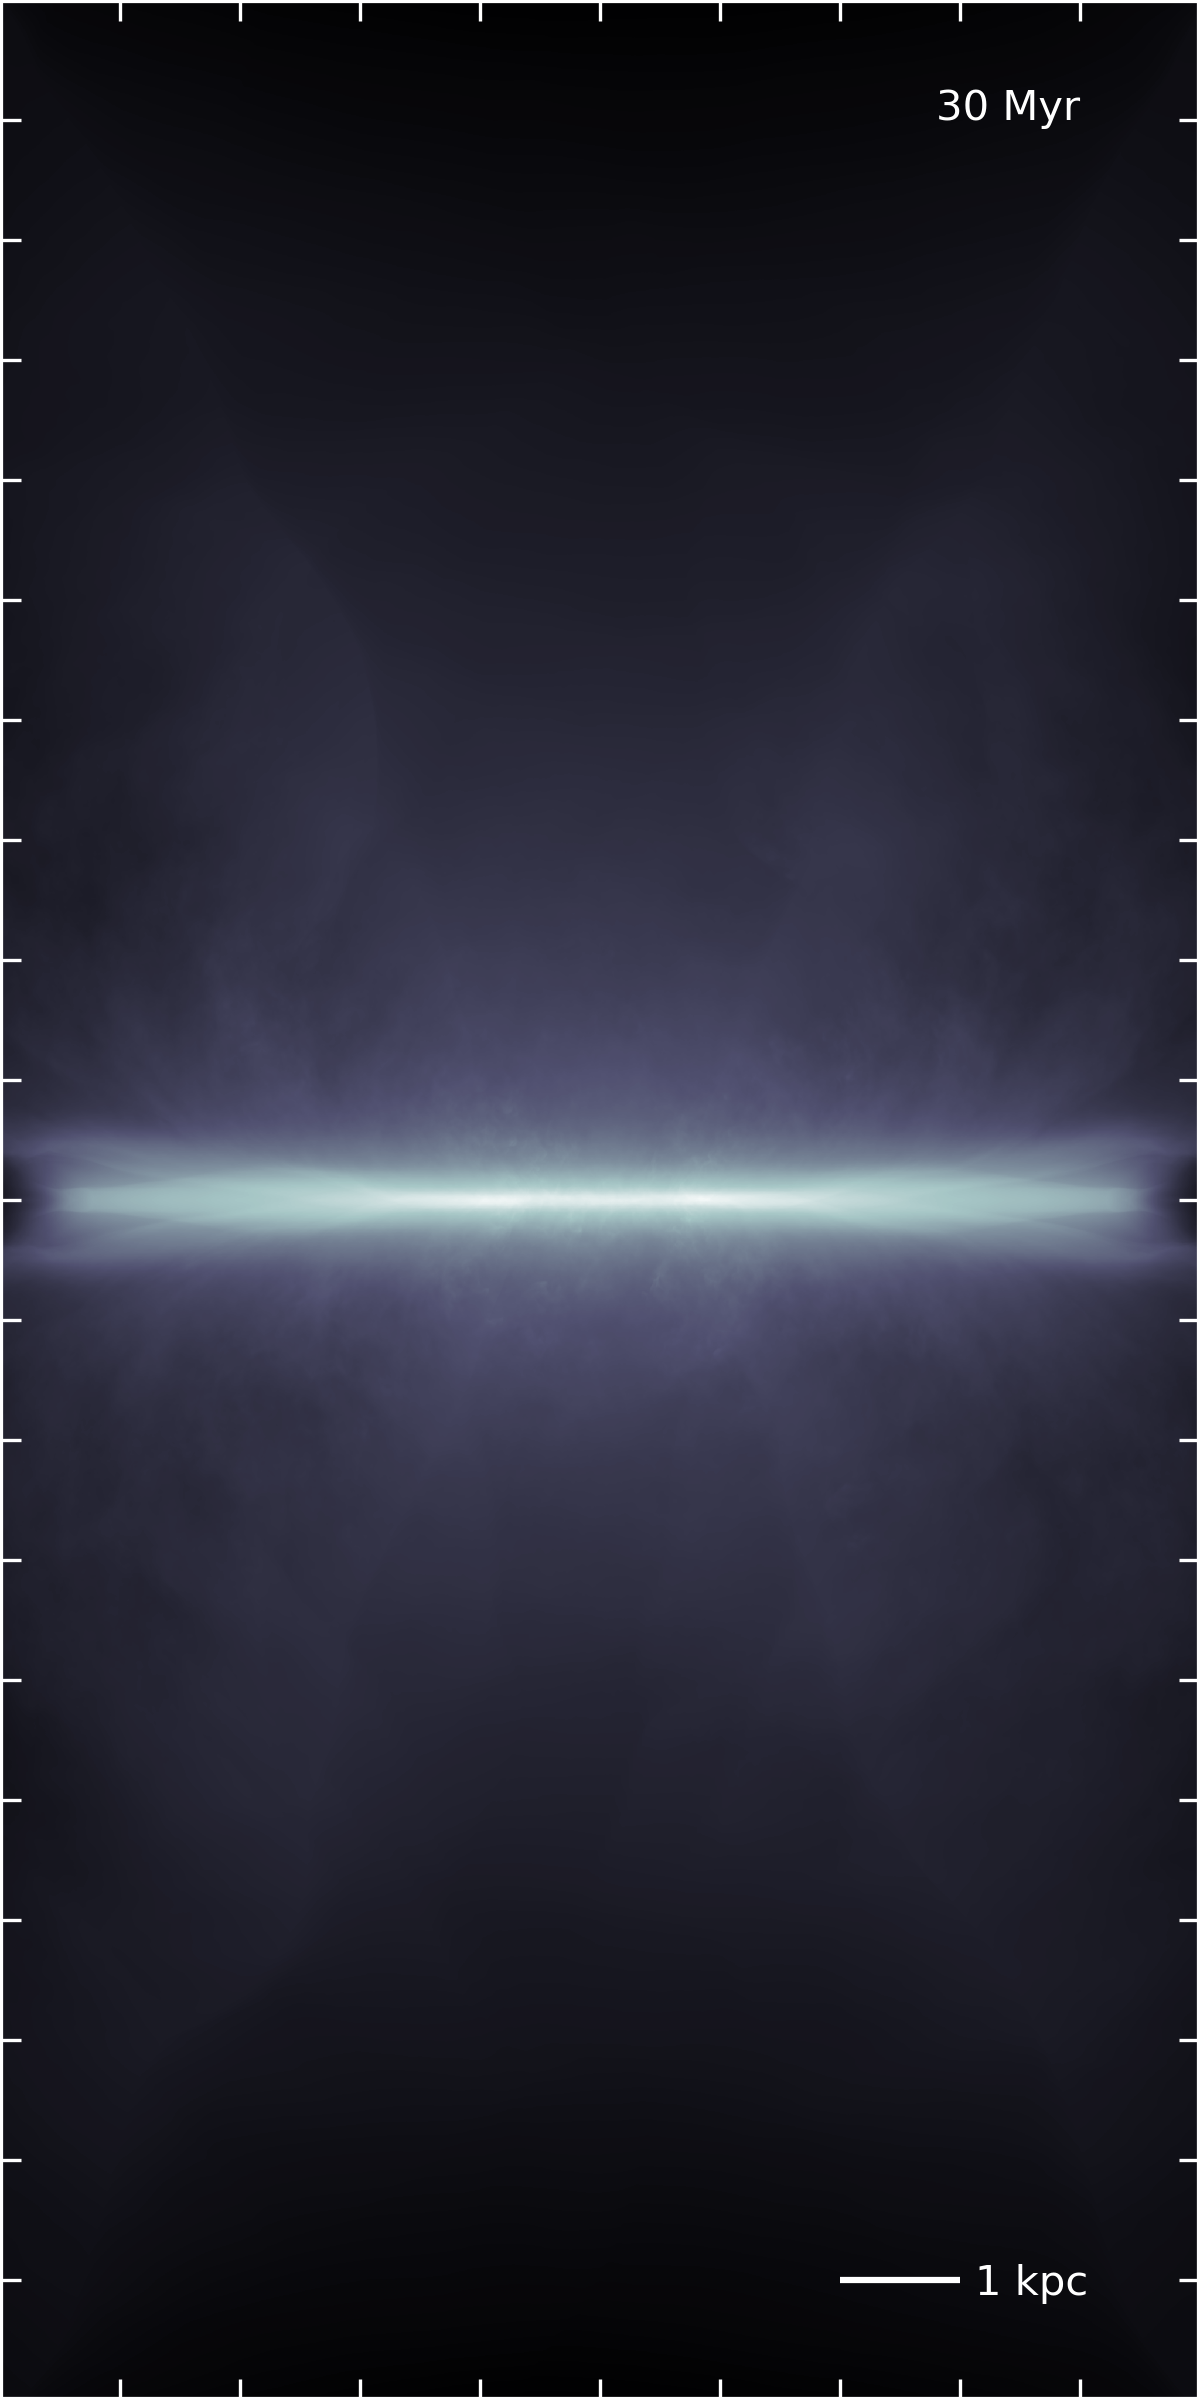
\includegraphics[width=0.35\linewidth]{M82_dxz.png}
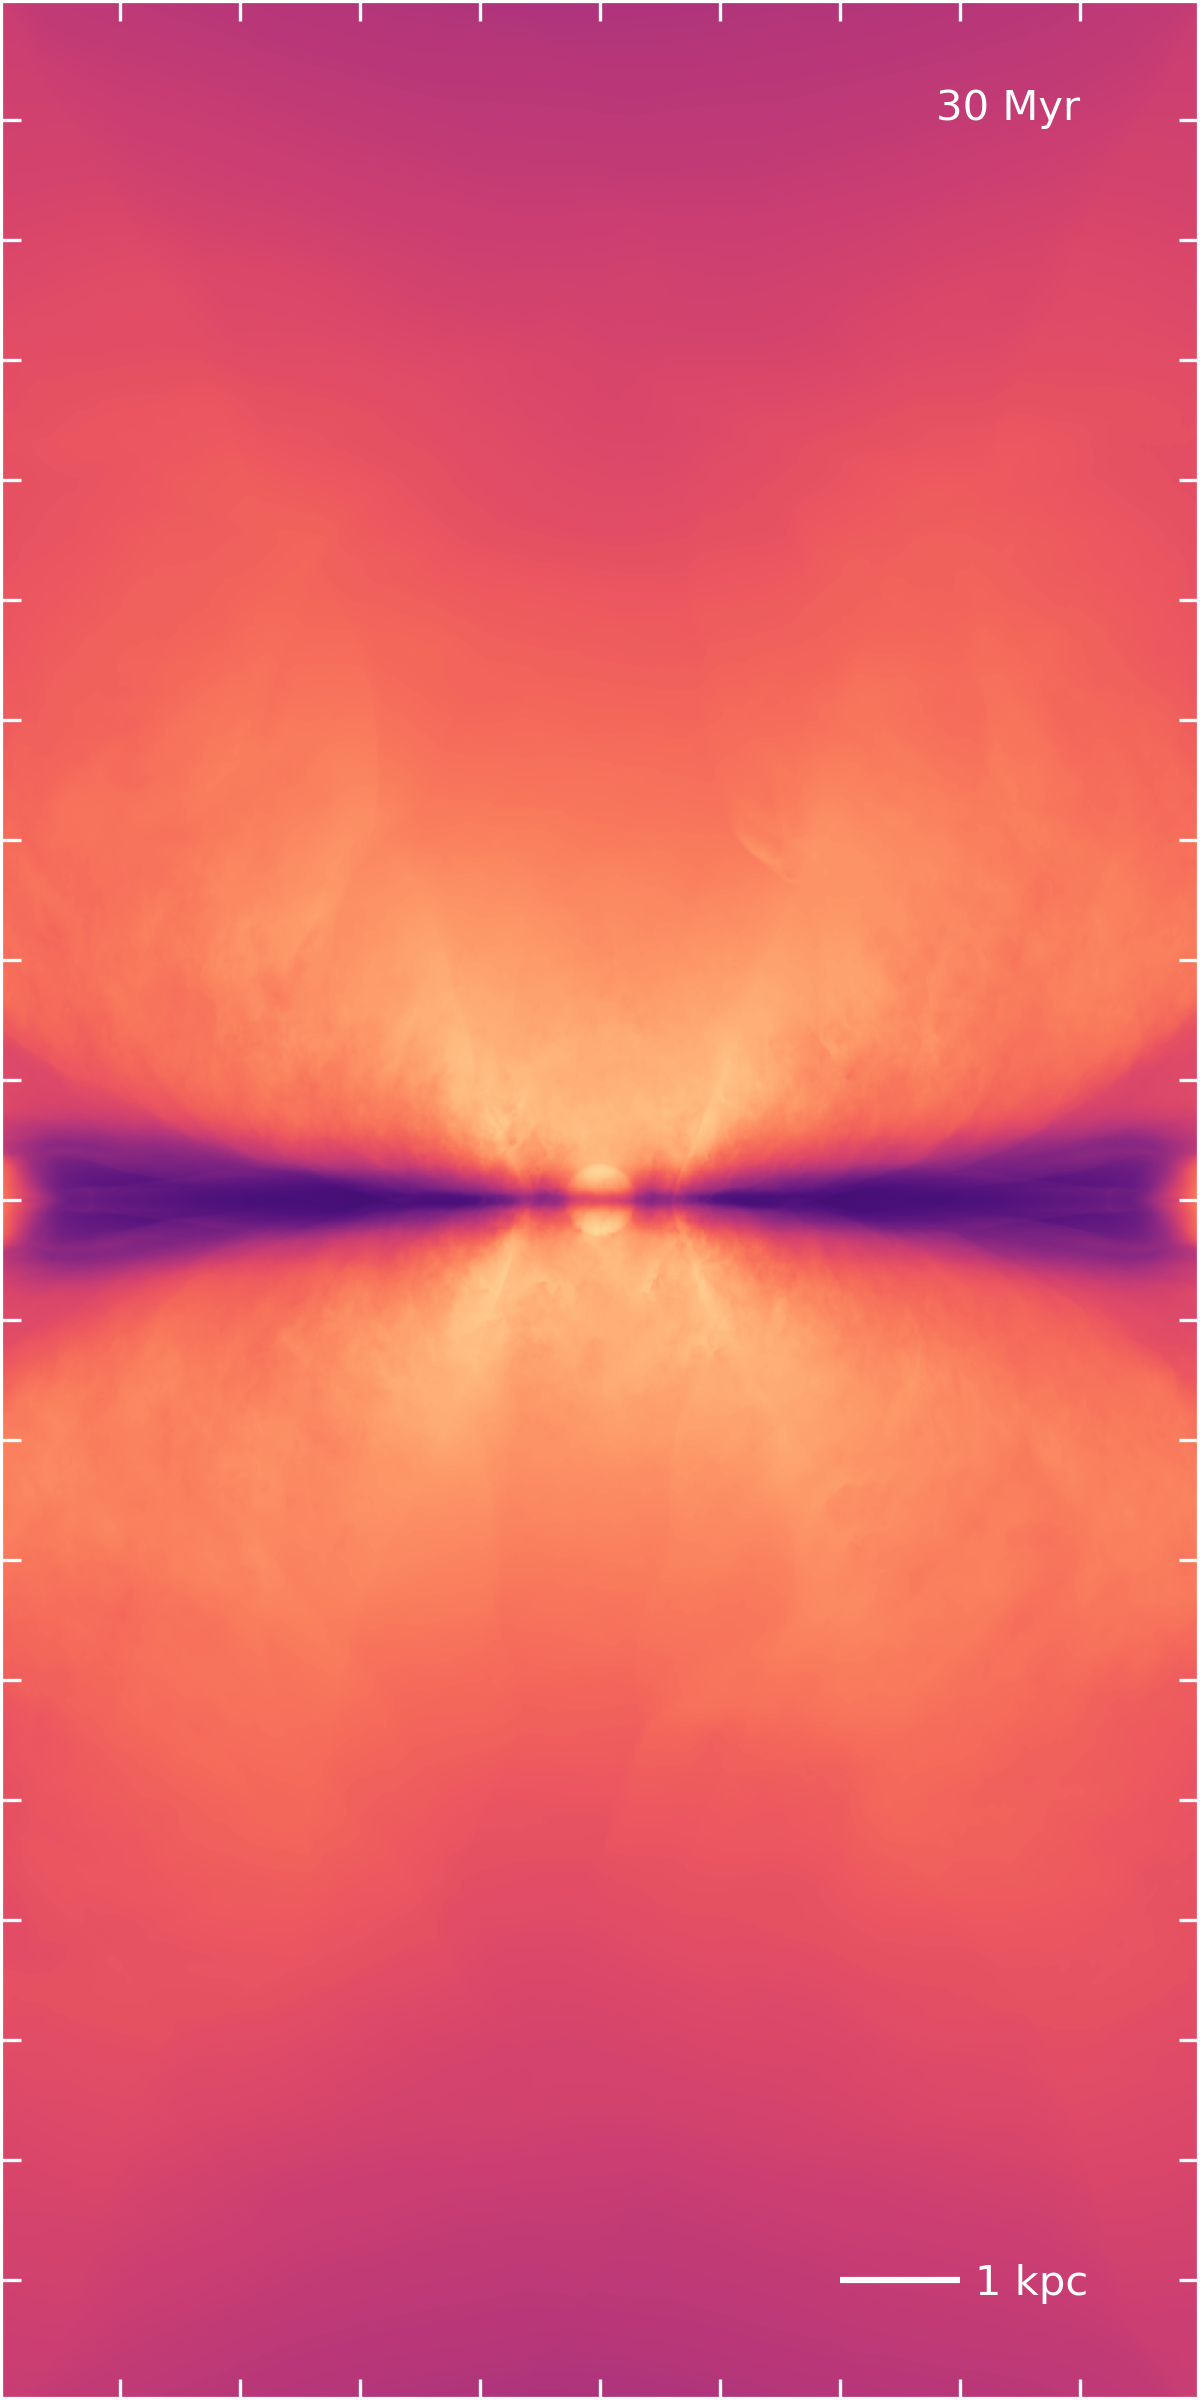
\includegraphics[width=0.35\linewidth]{M82_Txz.png}
\caption{Figure caption.}
\label{fig:adiabatic_2048}
\end{figure}

An advantage of our current simple feedback scheme is that it allows us to easily adjust the three parameters (SFR, mass-loading, and thermalization efficiency), in order to determine what range of parameters can cool on large scales. With our remaining 2017 allocation, we will be able to perform three production simulations with radiative cooling, that will explore the range of necessary mass-loading in order to achieve large-scale cooling in winds.

\subsubsection{Research Objective A: Simulate galactic outflows with numerical models that allow for supersonic wind velocities}

With the completion of Research Milestones A and B in Semester 1, we have also demonstrated that we have achieved the first research objective of our INCITE program: to simulate galactic outflows with numerical models that allow for supersonic wind velocities. While theoretical models had indicated that these starburst-driven winds should achieve supersonic velocities, the planar geometries employed in previous studies prevented winds from crossing the sonic point (see discussion in Martizzi et al. 2015). By simulating winds on a global scale, we have demonstrated that not only can winds achieve supersonic velocities, but that in scenarios where the injection rates can be well-approximated by the CC85 model, the large-scale features of those winds can be well-approximated by theory. We now turn to a discussion of the radiatively-cooling wind models that are the focus of our research program.

\subsubsection{Research Milestone C: Model the multiphase structure and radiative cooling of galactic outflows on $\sim$10 kpc scales}

Our 2016 INCITE proposal devotes all of Semester 2 to achieving Research Milestone C. As we are only a few weeks into Semester 2, we do not yet have all of the results, but we do have some early indications that the predictions of the theoretical models with radiative cooling will be born out in our production simulations. Figure \ref{fig:cooling_sim} shows the temperature in slices through the x-z plane for a calibration simulation (resolution $512\times512\times1024$ cells) with and without radiative cooling (left and right, respectively). Both plots were made after 22 million years of evolution. While the $10^4$ K disk is clearly visible on both simulations, the simulation with cooling also shows a large amount of gas between 2 - 5 kpc that has cooled to $10^4$ K. Early analysis of this simulation suggests that the velocities of this cool gas may be consistent with observations, which would make these the first simulations to successfully reproduce gas in this phase in large-scale galactic winds.

\begin{figure}[h]
\centering
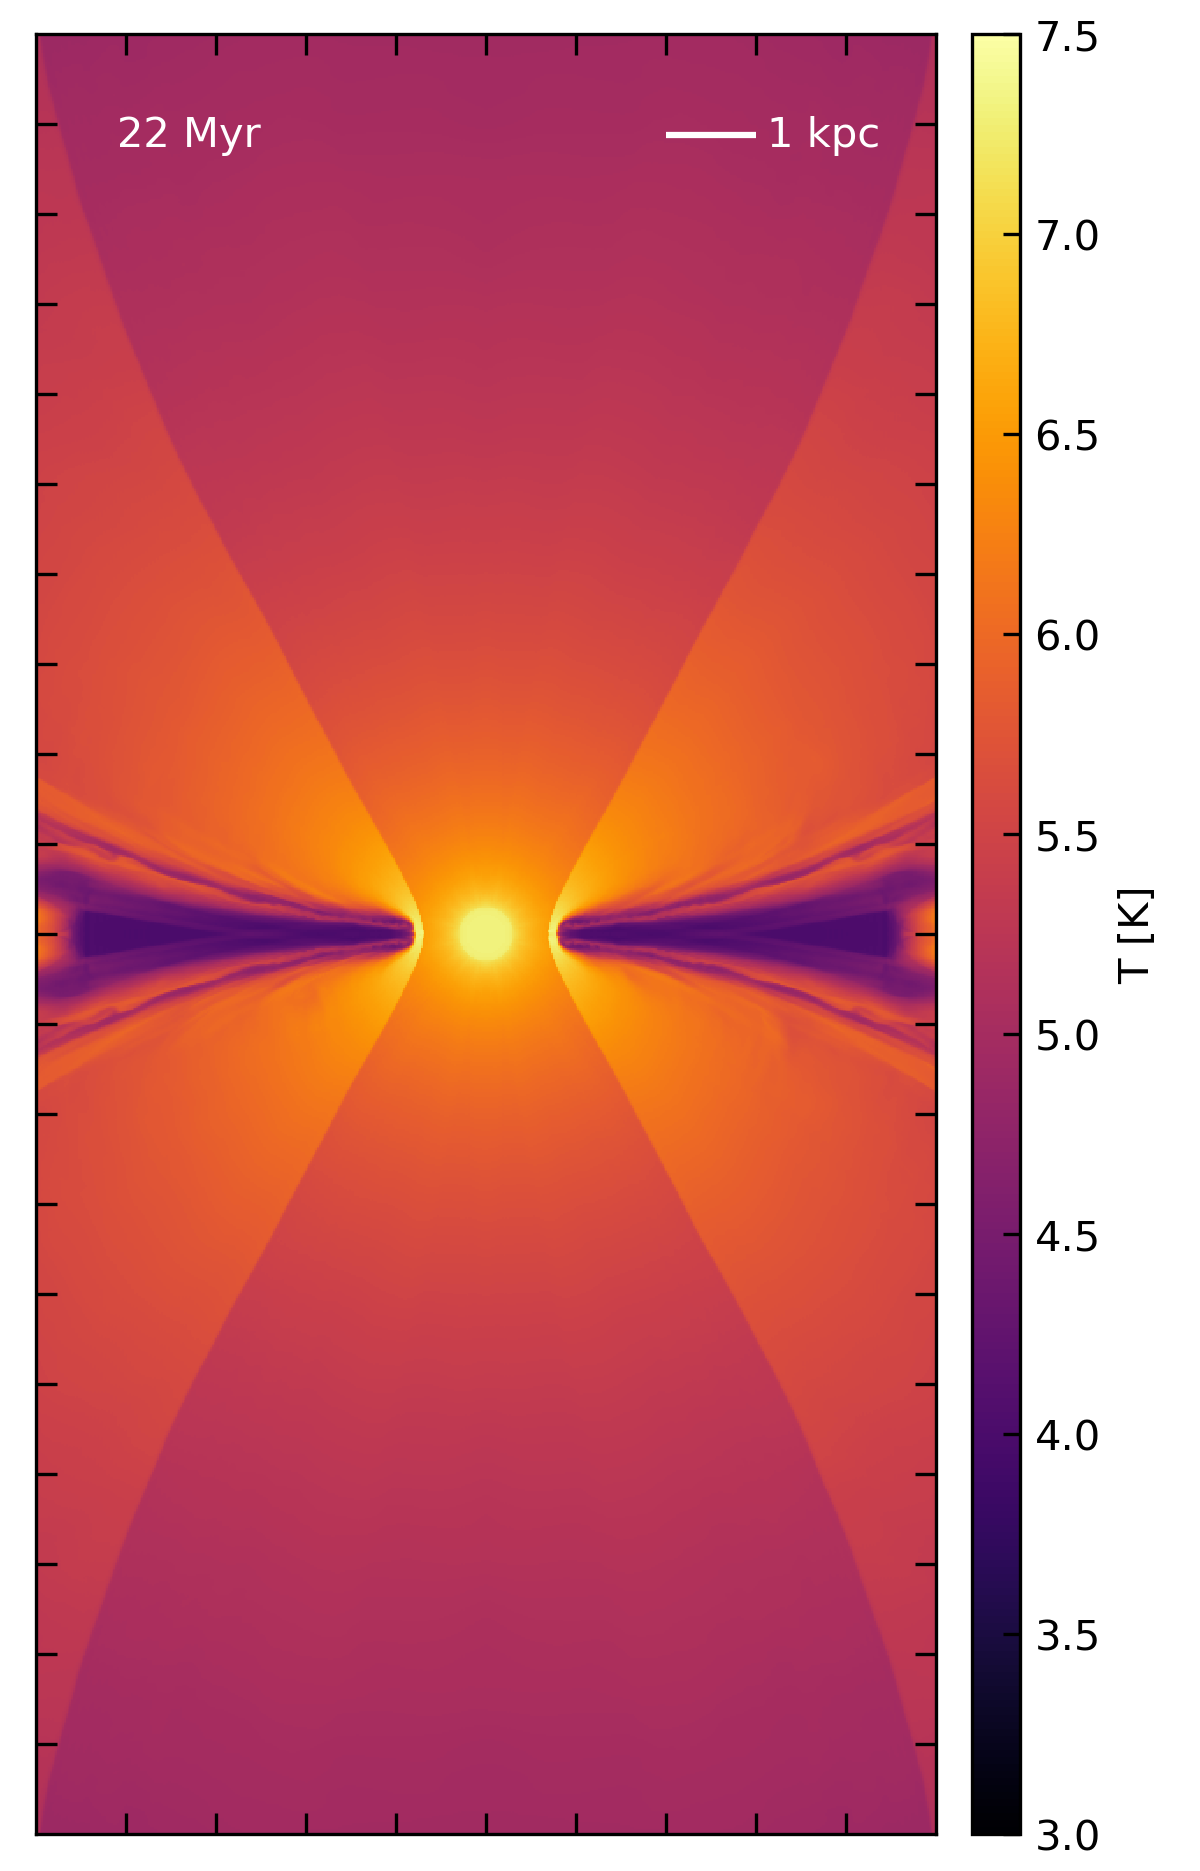
\includegraphics[width=0.35\linewidth]{Tslice_nocool.png}
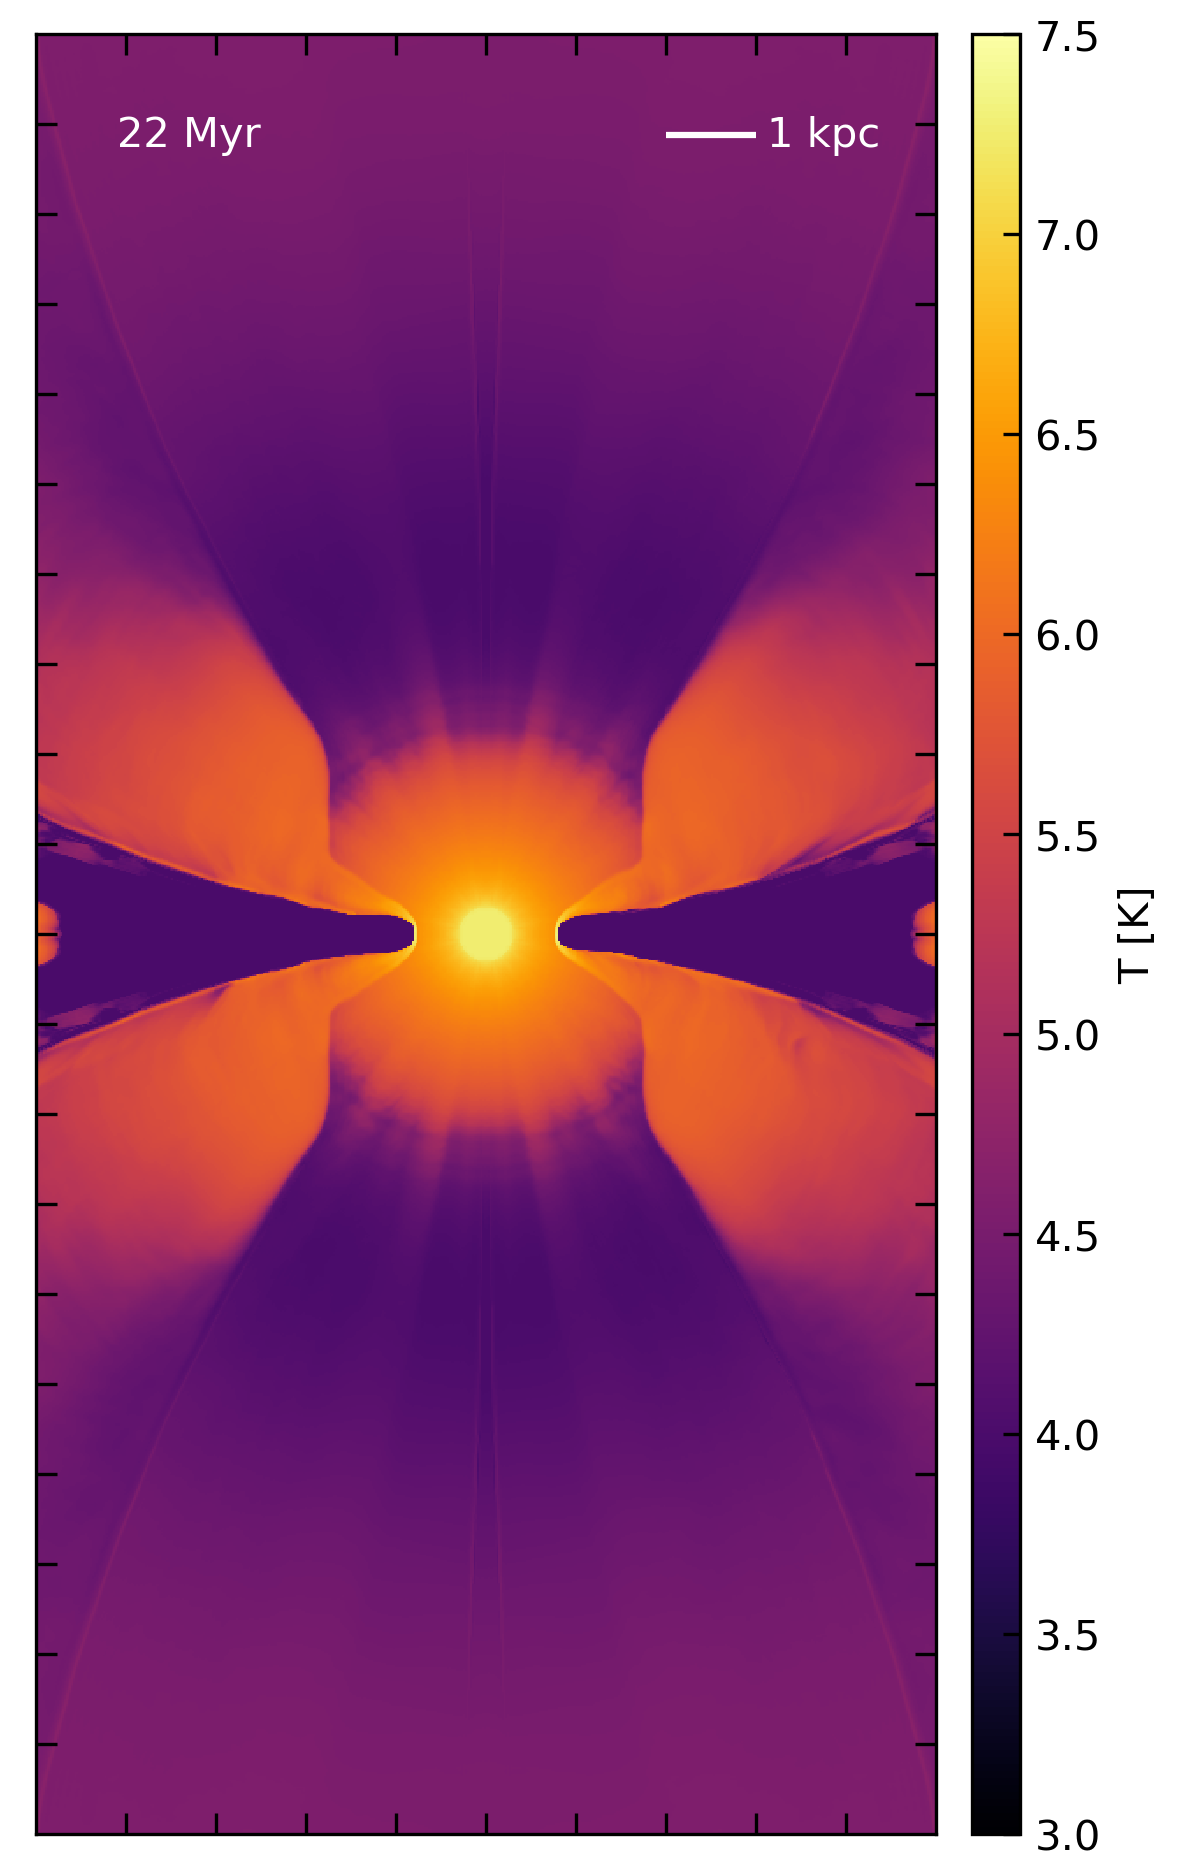
\includegraphics[width=0.35\linewidth]{Tslice_cool.png}
\caption{Figure caption.}
\label{fig:cooling_sim}
\end{figure}

We are currently finalizing the parameters for our production-scale radiative cooling wind simulations. Once we have decided on the appropriate parameters, we will run three production simulations with radiative cooling, which when compared with the adiabatic simulation presented in the previous section, will allow us to definitively answer the question posed by our Research Objective B: Quantify the importance of radiative cooling for the multiphase structure of observed galactic outflows.

\subsection{Allocation Use} 

Summarize your project's allocation use to date this year: percent of allocated core-hours used on each platform, job size distribution, number of users, etc. Associate the resource use with particular results where possible. Also summarize your project's projected use from now until the end of December (i.e., end of current allocation year): anticipated percent of allocated core-hours used on each platform, job size distribution, etc. Associate this resource usage with anticipated results. Do you expect your usage to be evenly distributed throughout the remainder of this year? If not, explain.

Insert paragraph(s).

\subsection{Application Parallel Performance} 

Summarize the performance (percent of peak, scalability) of your project's simulation tools used in the allocations this year. What progress was made in improving the application's performance on this architecture? What challenges (if any) remain? List the technical risks and challenges that were confronted by your project (overcome or not) this year. Were they anticipated?

Insert paragraph(s).


\subsubsection{Heading 3 (optional)}

Insert paragraph(s).


\subsection{Data Storage} 

What is the current cumulative size of stored data? What is your projection for the cumulative size of stored data at the end of the project? What tools and/or plans do you have to reduce the data? To share the data?

Insert paragraph(s).


\vspace{.08in}
\textbf{REFERENCES (optional, not included in the page count)}
\vspace{6pt}

References must be single-column format, 11 point, Arial or Times New Roman.

%\begin{enumerate}\itemsep0pt
%\item Doe, J.C., B.D. Smith, and L.M. Johnson. ``An article in a journal,'' \emph{The Journal} \textbf{32}(4): \\  46--52. \\


%\end{enumerate}

\end{document}
